% Colores
\definecolor{accblue}{RGB}{31,119,180}      % Quadratic (azul)
\definecolor{accgreen}{RGB}{44,160,44}      % Gaussian (verde tab:green)
\definecolor{accorange}{RGB}{255,127,14}    % Nuevo ACC (naranja tab:orange)

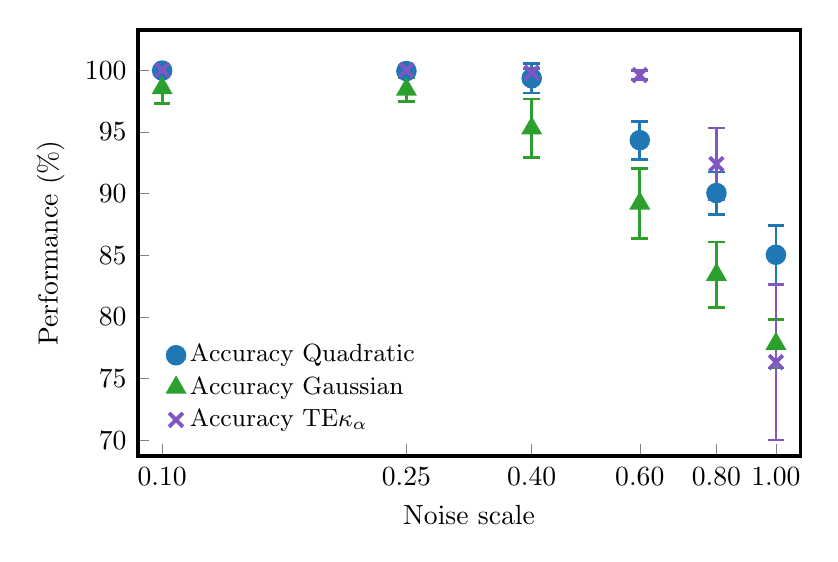
\begin{tikzpicture}
\begin{axis}[
    width=10cm, height=7cm,
    xlabel={Noise scale},
    ylabel={Performance (\%)},
    xmin=0.10, xmax=1.0,
    ymin=70, ymax=102,
    xmode=log, log basis x=10,
    xtick={0.10,0.25,0.40,0.60,0.80,1.00},
    xticklabels={0.10,0.25,0.40,0.60,0.80,1.00},
    ytick={70,75,80,85,90,95,100},
    xtick pos=bottom,
    ytick pos=left,
    legend style={draw=none, fill=none, font=\small},
    legend cell align=left,
    legend pos=south west,
    line width=1.4pt,
    mark size=3pt,
    enlarge x limits=0.04,
    enlarge y limits=0.04
]

% ===== Quadratic: mean ± SD muestral (n=5) =====
% Q1: 96.9, 98.4, 97.8, 95.4, 92.7, 87.9
% Q2: 99.9, 99.96, 97.6, 94.1, 90.5, 83.7
% Q3: 99.9, 99.93, 98.94, 92.0, 88.2, 82.3
% Q4: 99.97, 98.9, 97.2, 94.1, 89.7, 87.1
% Q5: 99.9, 99.98, 997.8, 96.0, 89.1, 84.2
% => mean (%): 99.26, 99.20, 97.76, 94.32, 90.04, 85.04
%    SD (muestral): 1.32, 0.56, 0.43, 1.54, 1.71, 2.37
% Nota: en x=0.10 capamos la barra superior para no exceder 100% (y+ = 0.74).
\addplot+[
    only marks,
    color=accblue,
    mark=*,
    mark options={solid, fill=accblue},
    error bars/.cd,
      y dir=both, y explicit,
      error bar style={line width=1pt},
      error mark=|,
      error mark options={mark size=3pt, line width=1pt}
] coordinates {
    (0.10, 99.96) +- (0, 0.04)
    (0.25, 99.92) +- (0, 0.04)
    (0.40, 99.34) +- (0, 1.20)
    (0.60, 94.32) +- (0, 1.54)
    (0.80, 90.04) +- (0, 1.71)
    (1.00, 85.04) +- (0, 2.37)
};
\addlegendentry{Accuracy Quadratic}

% ===== Gaussian: mean ± SD muestral (n=5), VERDE triangulitos =====
% Corridas usadas (en %):
% G1 (nuevo): 97.5, 97.1, 91.7, 86.0, 80.5, 77.1
% G2:         98.5, 97.8, 94.4, 87.5, 82.6, 75.6
% G3:         97.1, 98.6, 95.7, 89.0, 82.6, 78.2
% G4:         99.8, 99.0, 96.8, 90.1, 83.7, 77.3
% G5:         99.8, 99.6, 97.8, 93.4, 87.7, 80.9
% => mean (%): 98.54, 98.42, 95.28, 89.20, 83.42, 77.82
%    SD (muestral): 1.26, 0.99, 2.37, 2.81, 2.66, 1.96
\addplot+[
    only marks,
    color=accgreen,
    mark=triangle*,
    mark options={solid, fill=accgreen},
    error bars/.cd,
      y dir=both, y explicit,
      error bar style={line width=1pt},
      error mark=|,
      error mark options={mark size=3pt, line width=1pt}
] coordinates {
    (0.10, 98.54) +- (0, 1.26)
    (0.25, 98.42) +- (0, 0.99)
    (0.40, 95.28) +- (0, 2.37)
    (0.60, 89.20) +- (0, 2.81)
    (0.80, 83.42) +- (0, 2.66)
    (1.00, 77.82) +- (0, 1.96)
};
\addlegendentry{Accuracy Gaussian}

% % ===== Nuevo ACC (naranja): por ahora SOLO 1 punto =====
% ===== Accuracy Iván (σ fijo = 0.25): mean ± SD (n=3), NARANJA =====

\definecolor{accpurple}{HTML}{7E57C2}

\addplot+[
  only marks,
  mark=x,
  mark size=3.5pt,
  color=accpurple,
  line width=1.4pt,
  error bars/.cd,
    y dir=both, y explicit,
    error bar style={line width=1pt, color=accpurple},
    error mark=|,
    error mark options={mark size=3pt, line width=1pt, color=accpurple}
] coordinates {
  (0.10, 100.00) +- (0, 0.00)
  (0.25, 100.00) +- (0, 0.00)
  (0.40,  99.79) +- (0, 0.36)
  (0.60,  99.59) +- (0, 0.36)
  (0.80,  92.39) +- (0, 2.92)
  (1.00,  76.34) +- (0, 6.31)
};
\addlegendentry{Accuracy TE$\kappa_\alpha$}


\end{axis}
\end{tikzpicture}
